\section{Satellite galaxies around a massive central}

General code used in this exercise is:
\lstinputlisting[firstnumber=1, firstline=1, lastline=124]{Q1.py}



\subsection{a}

We use golden section search to find the maximum $N(x)$ for $x\in[0,5)$.
We implemented the golden section search algorithm as a minimization algorithm,
so instead of maximizing $N(x)$ we minimize $-N(x)$.
The algorithm requires us to choose an initial bracket.
We plot the function $N$ with the given parameters and domain, the result of which is shown in Figure \ref{fig:max},
from which we see that (0, 0.5, 1) forms a good bracket (because $N(0)<N(0.5)$ and $N(1)<N(0.5)$). 
Using this bracket and applying the minimization algorithm, we find the maximum which is also indicated in Figure \ref{fig:max}.

The code used is:
\lstinputlisting[firstnumber=1, firstline=128, lastline=185]{Q1.py}

The resulting maximum is:
\lstinputlisting[firstnumber=1, firstline=1, lastline=1]{output_Q1.txt}

\begin{figure}[h!]
    \centering
    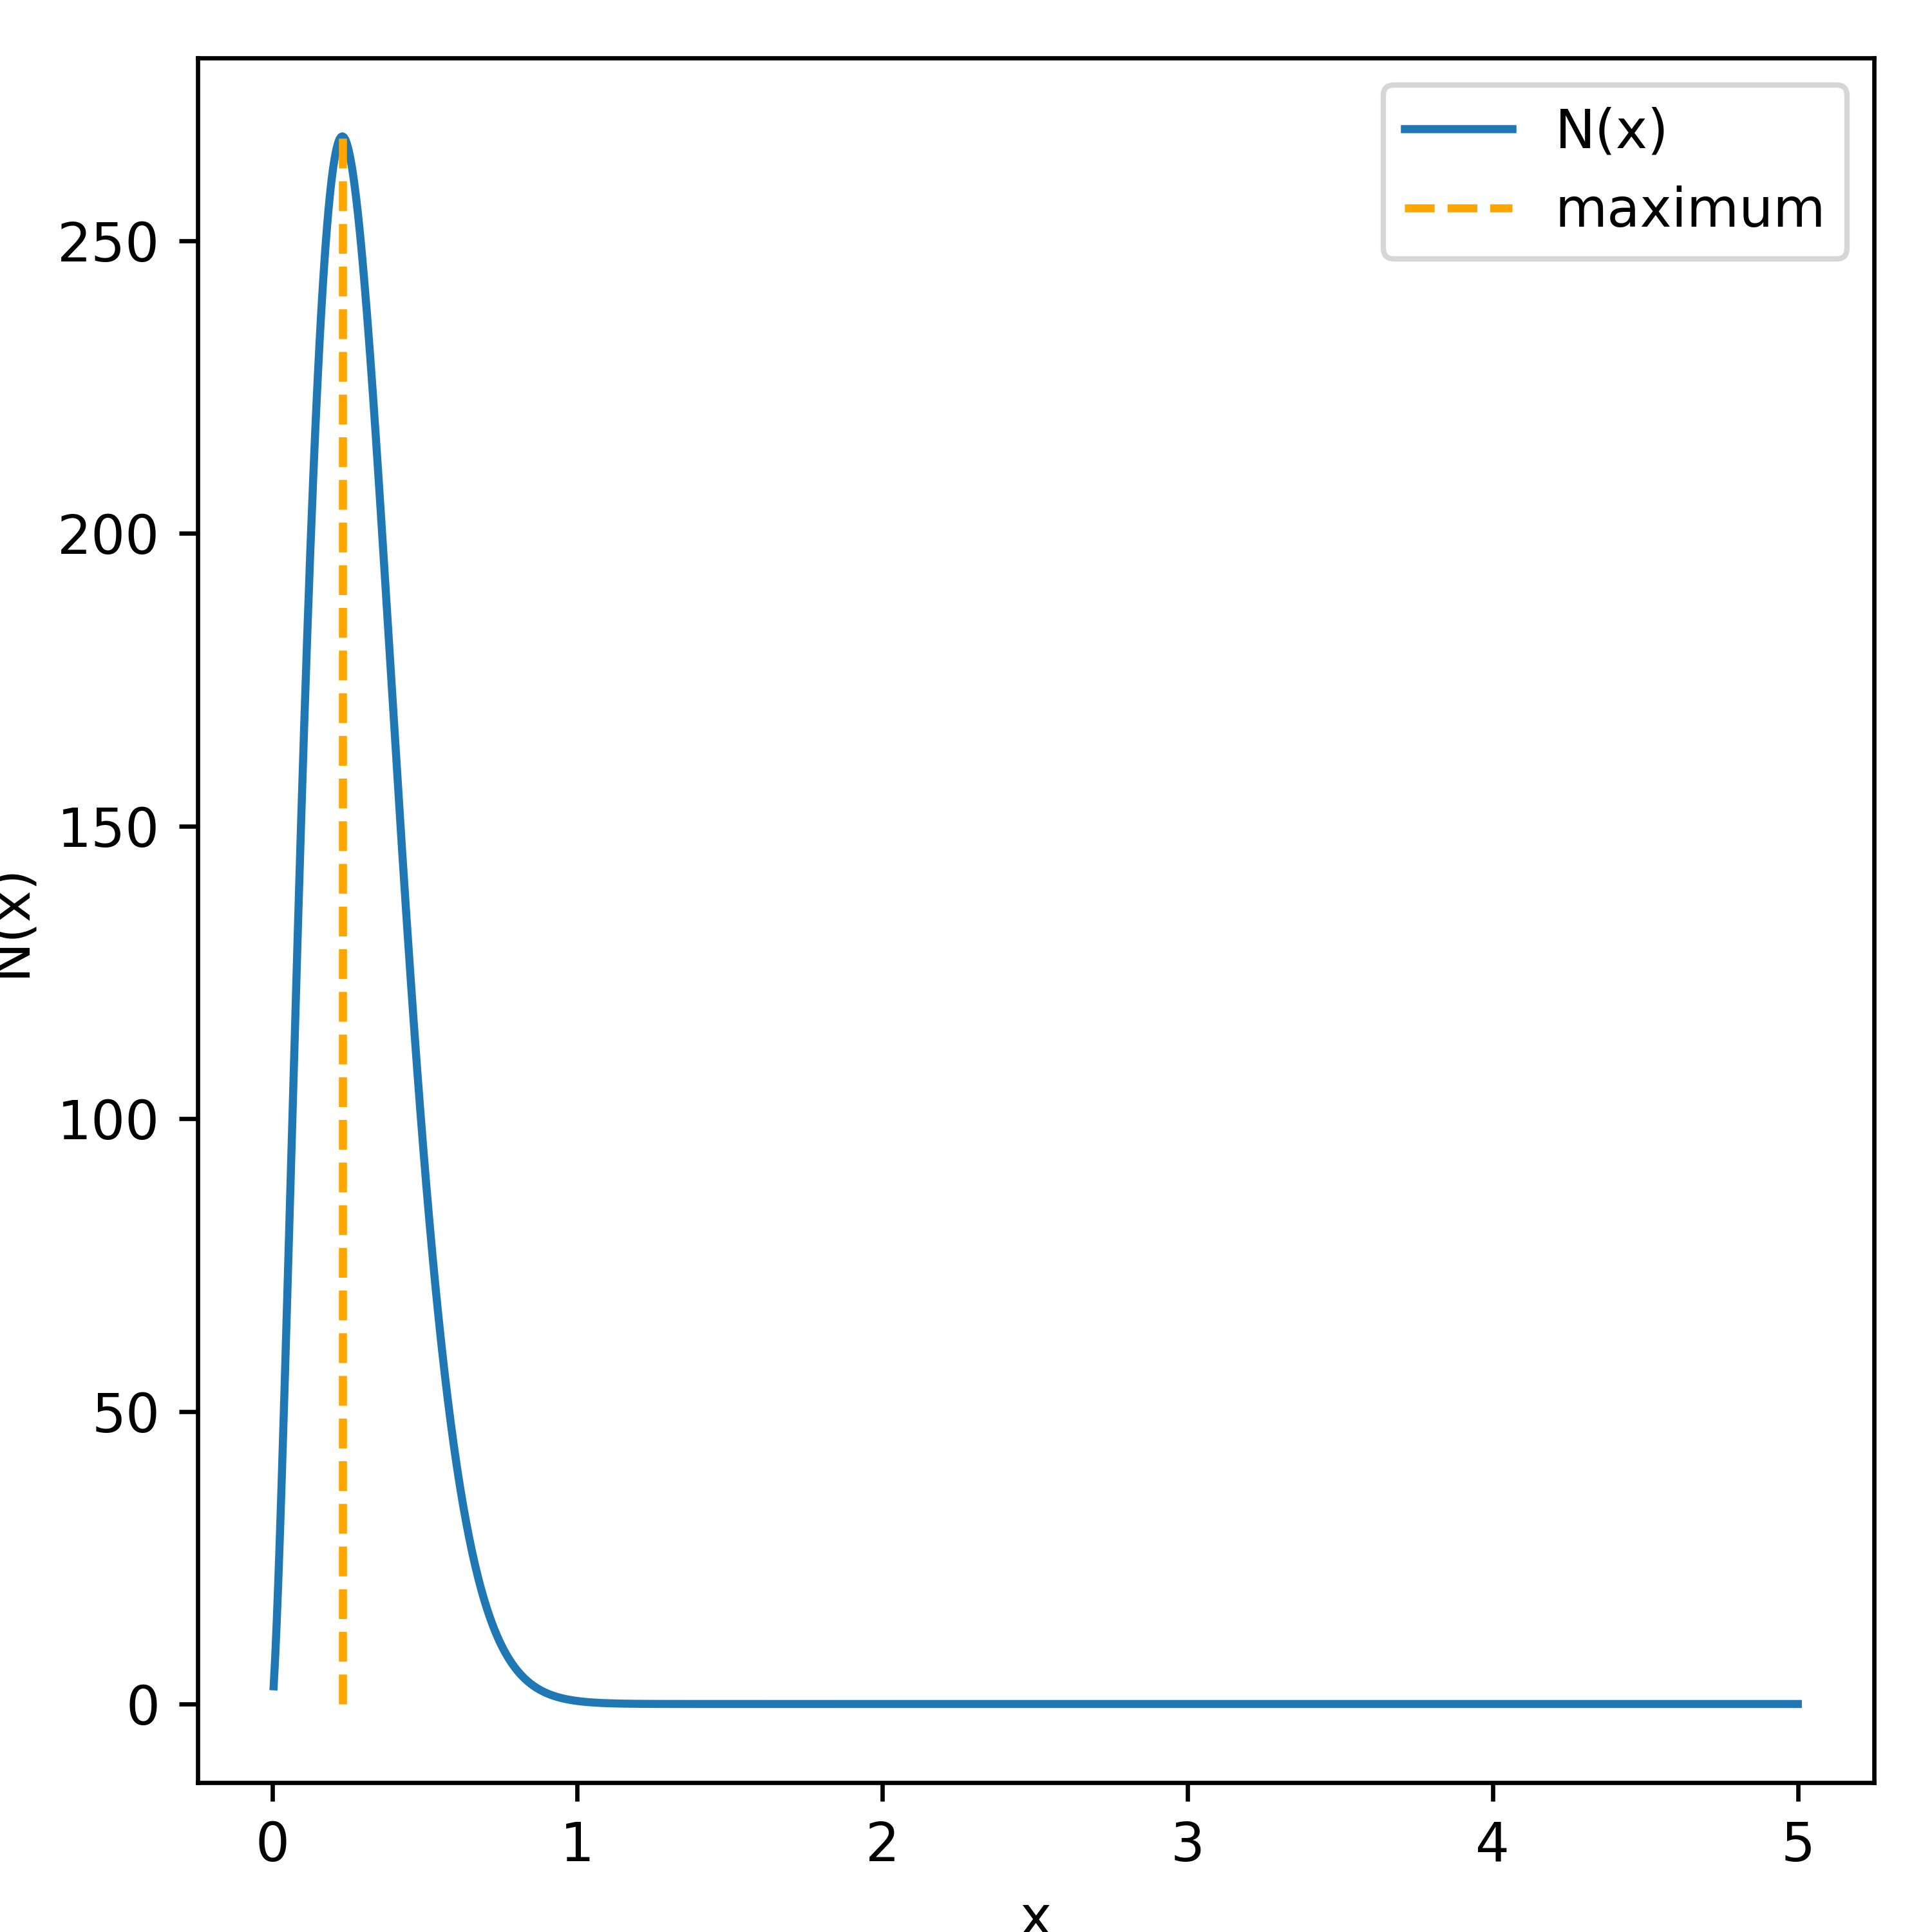
\includegraphics[width=0.5\linewidth]{./my_solution_1a.png}
    \caption{The function $N(x)$ is plotted for $x\in[0,5)$. The found maximum is indicated with a vertical line.
    Indeed, this corresponds to the maximum of the function.}
    \label{fig:max}
\end{figure}



\subsection{b}

We choose to use 50 radial bins in log space, as more bins gives more accurate information on the function so a tighter constraint on the model fit, 
which means that the minimum will be more easily found.
As range we choose to use $xmin=1e^{-4}$ as in the previous assignment, such that we do not have to deal with division by zero but at the same time do keep
x small. We considered using the minimal radius within the dataset as $xmin$, but this would mean we do not take the fact that we find no satellite galaxies below
this radius into account in the model, while this is important information that should not be left out. For the maximal radius we choose to use the maximal radius found in the dataset.

We calculate $\langle N_{sat}\rangle$ by dividing the total number of radii by the number of halos within the dataset. 
The binned data $N_i$ is also divided by the number of halos.

We have that 
\begin{align*}
    \tilde{N_i} 
    &= 4\pi\int_{x_i}^{x_{i+1}} n(x)x^2 \text{d}x\\
    &= 4\pi\int_{x_i}^{x_{i+1}} A \langle N_{sat} \rangle (\frac{x}{b})^{a-3}\exp{-(\frac{x}{b})^c}x^2 \text{d}x\\
    &= \frac{4\pi\int_{x_i}^{x_{i+1}} \langle N_{sat} \rangle (\frac{x}{b})^{a-3}\exp{-(\frac{x}{b})^c}x^2 \text{d}x}{4\pi \int_{0}^{5} (\frac{x}{b})^{a-3}\exp{-(\frac{x}{b})^c}x^2 \text{d}x}\\
    &= \frac{\langle N_{sat} \rangle\int_{x_i}^{x_{i+1}} (\frac{x}{b})^{a-3}\exp{-(\frac{x}{b})^c}x^2 \text{d}x}{\int_{0}^{5} (\frac{x}{b})^{a-3}\exp{-(\frac{x}{b})^c}x^2 \text{d}x}.
\end{align*}
The integrals are computed using the midpoint extended Romberg method which we implemented in the previous assignment. We use this form to compute
\begin{align*}
    \chi^2 &= \sum \frac{(N_i-\tilde{N_i})^2}{\tilde{N_i}},
\end{align*}
where the sum is over the bins.

To minimize this $\chi^2$ we use the downhill simplex method with a maximum of 500 steps, as we found that in most cases it will converge within a few hundred steps and otherwise
take ages (get stuck?) to converge. The sorting within the downhill simplex method is done using quicksort which we implemented in the previous assignment.
We have found that the found minimum depends on the choice of initial simplex.
Therefore, we use a few different initial simplexes, around the parameters $a=2.4, b=0.25, c=1.6$, and repeat the method
for each of these, after which we take the parameters that provide the lowest $\chi^2$ over all.
The resulting fits are shown in Figure \ref{fig:1b}. By visual inspection the fits look good.

The code used is:
\lstinputlisting[firstnumber=1, firstline=200, lastline=340]{Q1.py}

\begin{figure}[h!]
    \centering
    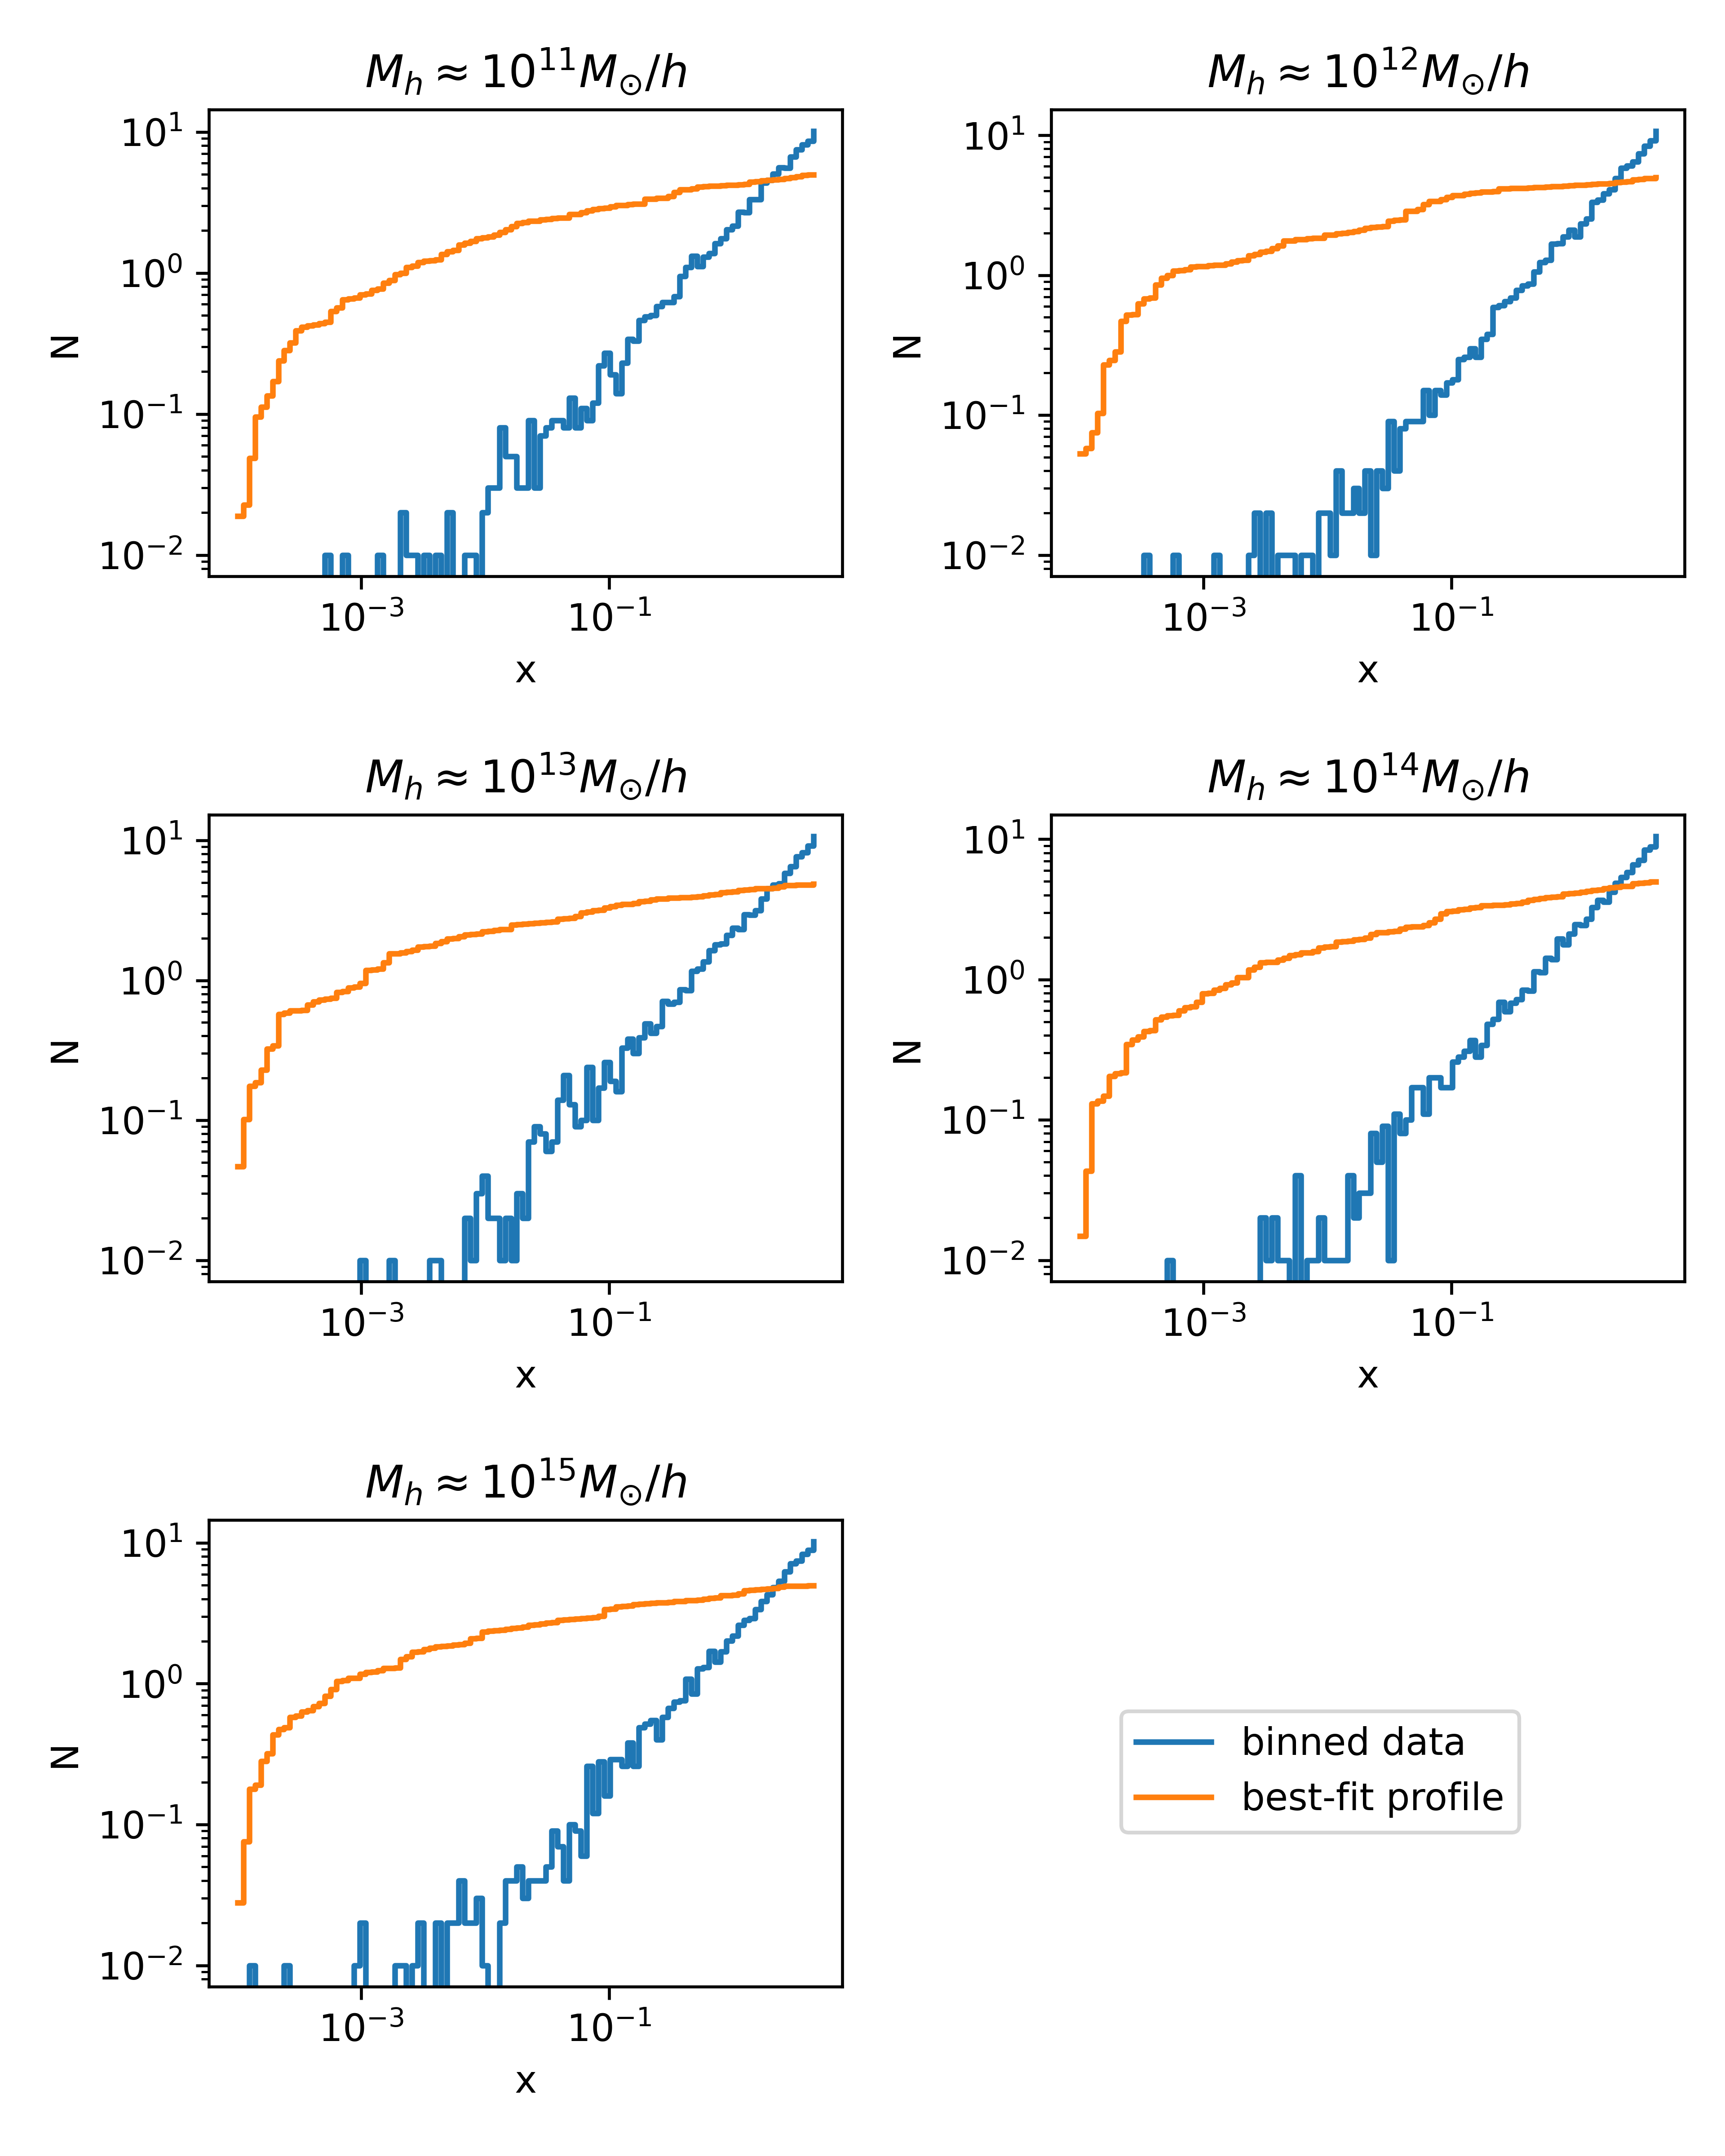
\includegraphics[width=0.9\linewidth]{./my_solution_1b.png}
    \caption{In each of the panels a different binned dataset (blue) and corresponding model fit (orange) is shown. The used model is Gaussian, resulting in a $\chi^2$ fit.
    Note that the axes are in log space, such that the obvious and seemingly weird gaps at lower radii are caused by for example missing only one or two count in that particular bin.
    The fits look good by visual inspection.}
    \label{fig:1b}
\end{figure}

The corresponding fit values for the Gaussian fit are:
\lstinputlisting[firstnumber=1, firstline=2, lastline=7]{output_Q1.txt}



\subsection{c}

The Poisson log-likelihood for $\tilde{N_i}$ model counts and $N_i$ mean observed counts per bin is
\begin{align*}
    -\ln(\mathcal{L}(a,b,c))=-\sum (N_i\ln(\tilde{N_i})-\tilde{N_i})
\end{align*}
where the sum is again over the same bins as for b.
We now use the same method as for b to minimize the -log likelihood. The resulting fits are shown in Figure \ref{fig:1c}.

The code used is:
\lstinputlisting[firstnumber=1, firstline=344, lastline=414]{Q1.py}

\begin{figure}[h!]
    \centering
    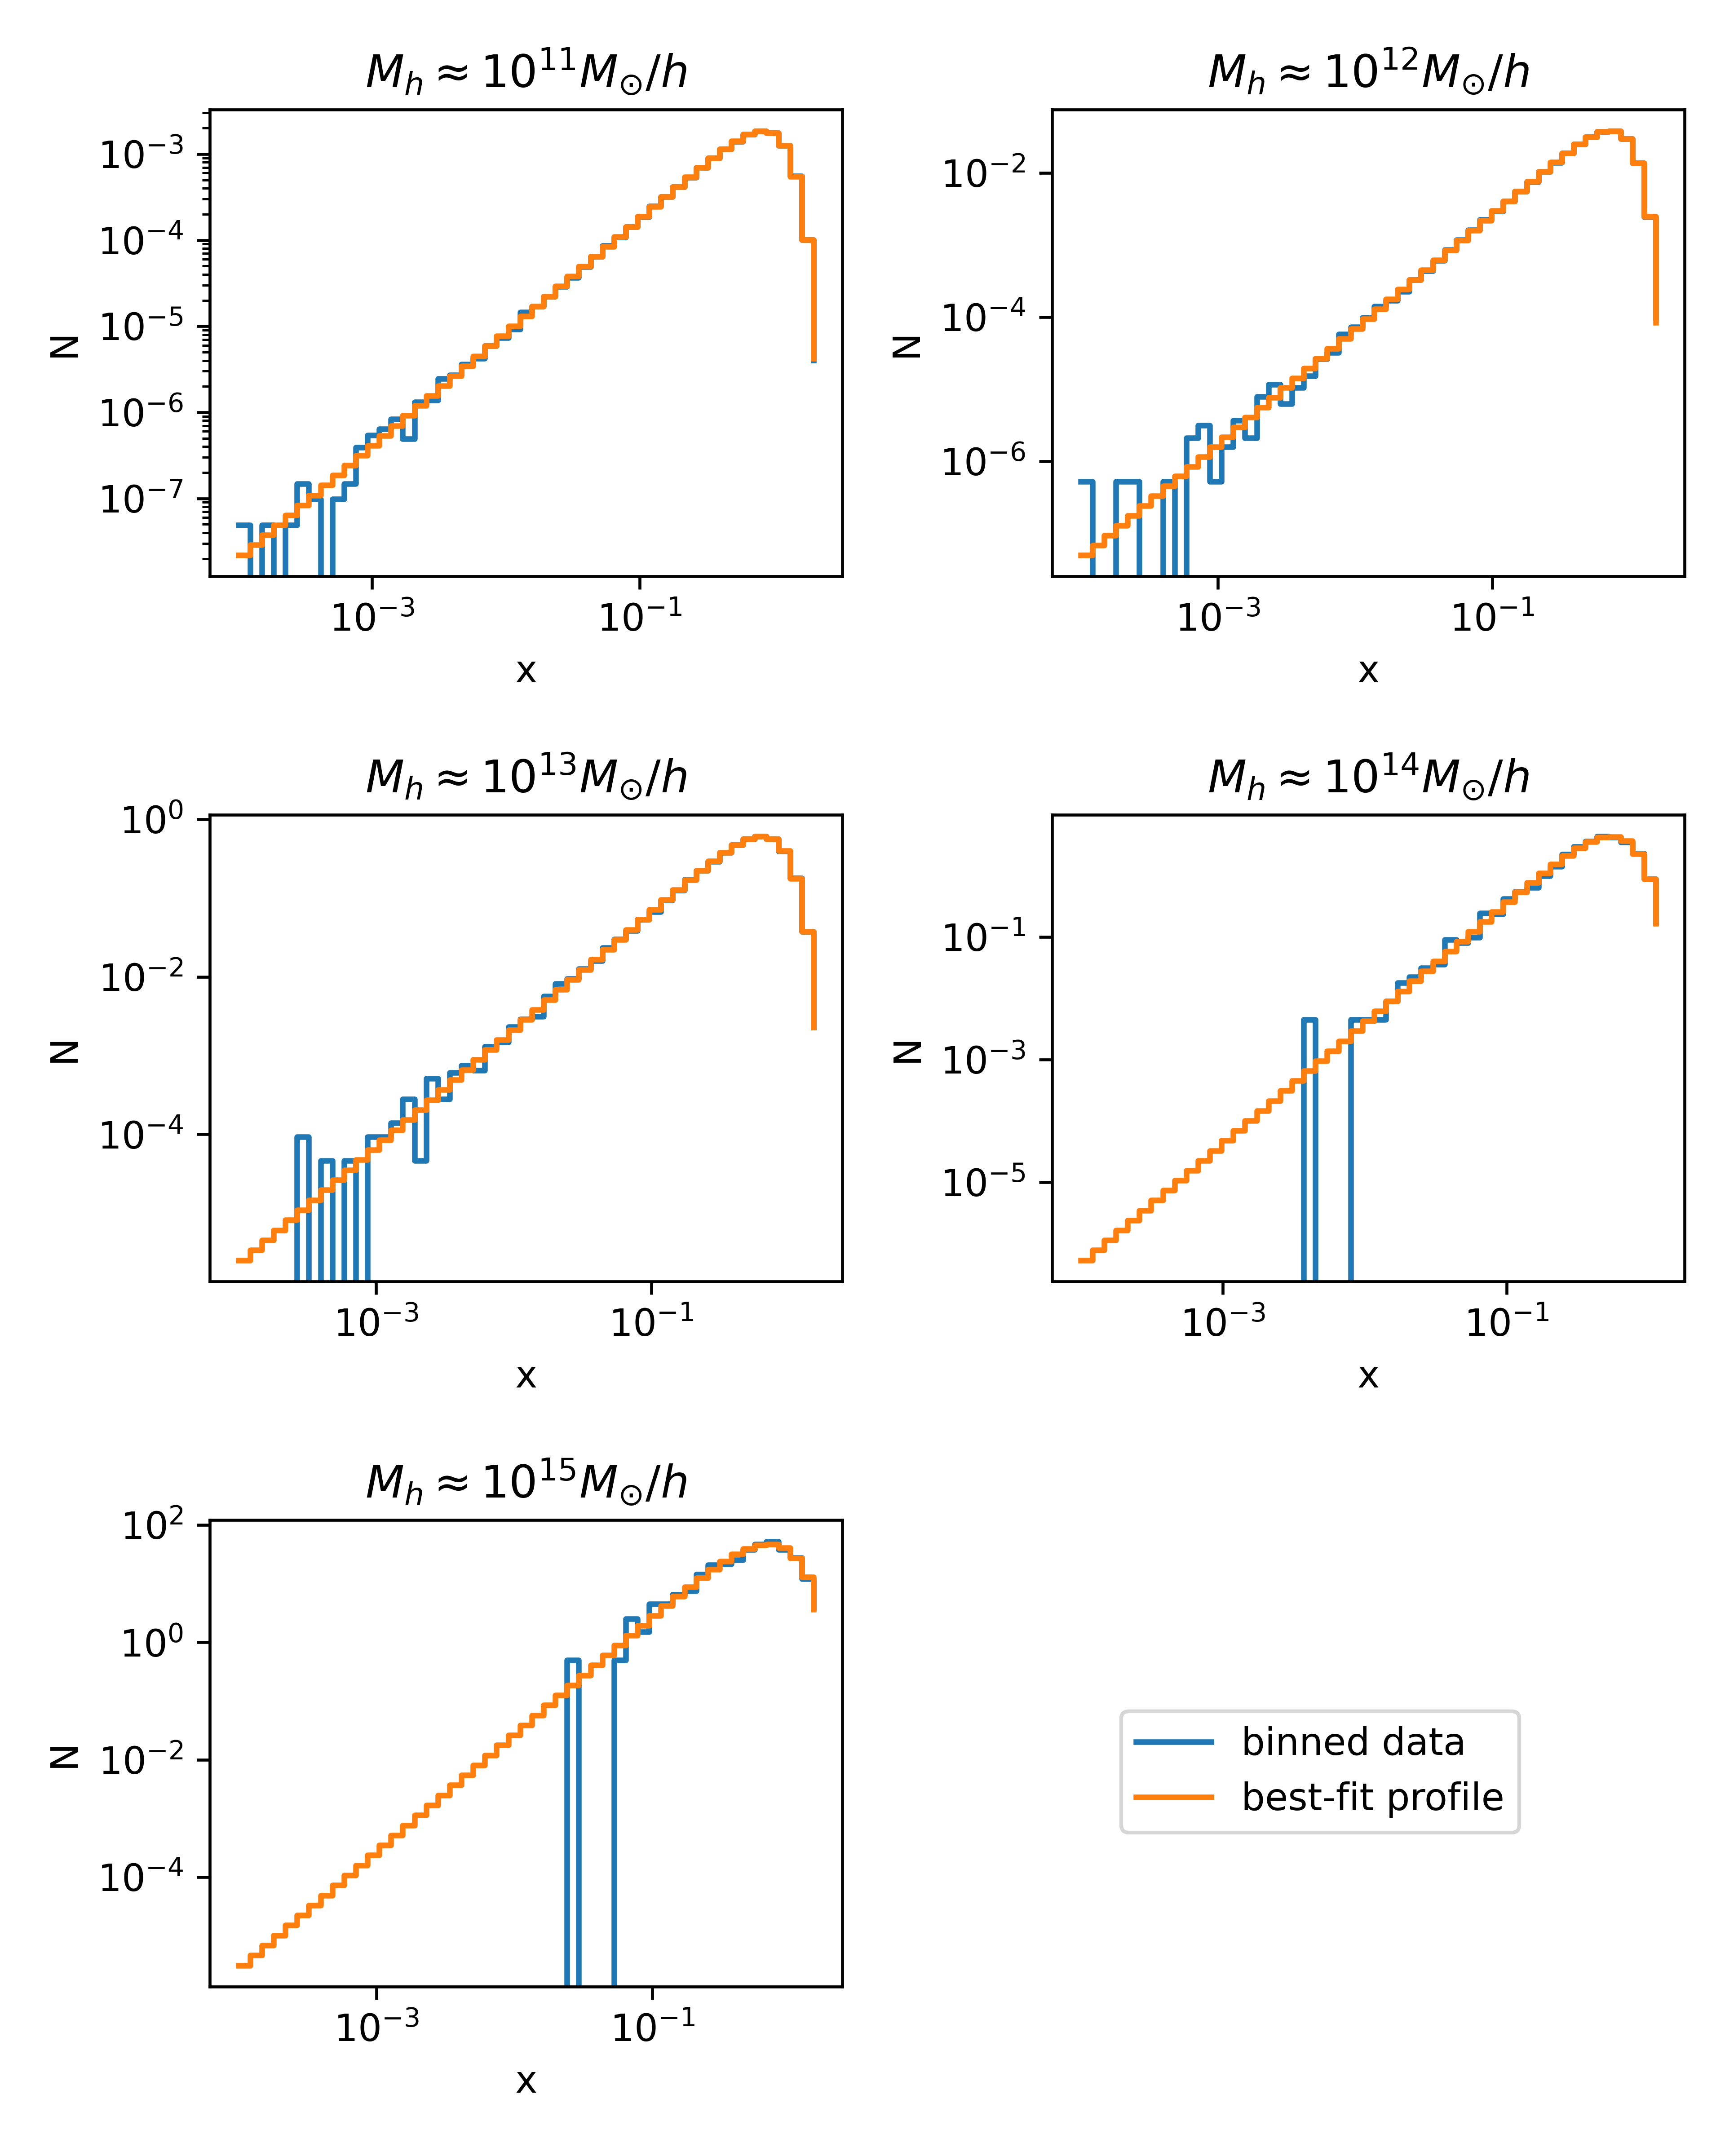
\includegraphics[width=0.9\linewidth]{./my_solution_1c.png}
    \caption{In each of the panels a different binned dataset (blue) and corresponding model fit (orange) is shown. The used model is Poissonian.
    Note that the axes are in log space, such that the obvious and seemingly weird gaps at lower radii are caused by for example missing only one or two count in that particular bin.
    The fits look good by visual inspection.}
    \label{fig:1c}
\end{figure}

The corresponding fit values for the Poisson fit are:
\lstinputlisting[firstnumber=1, firstline=8, lastline=13]{output_Q1.txt}



\subsection{d}

We calculate the G-statistic for both the Gaussian and Poissonian method.
The $G$-statistic is calculated by 
\begin{align*}
    G = 2\sum O_i \ln(\frac{O_i}{E_i}),
\end{align*}
where $O_i$ is the observed number of satellites in each bin (as an integer, so we multiply by the number of halos), and $E_i$ is the expected number of satellites in each bin according
to the model. $E_i$ must be a positive number, which it is in each bin. Furthermore, if $O_i=0$ in certain bins, we do not take the contribution of these bins into account as $O_i\ln(O_i)\to 0$.
To compute the significance $Q$ of $G$ we have that 
\begin{align*}
    Q &= 1-P(G,k)\\
    &= 1-\frac{\gamma(\frac{k}{2},\frac{G}{2})}{\Gamma(\frac{k}{2})},
\end{align*} 
which is the regularized lower incomplete gamma function. Here $k$ is the number of degrees of freedom,
which is equal to the number of bins minus the number of parameters (3) in this case. 

The results for each of the datasets are shown in the tables of results for b and c.
We find that the values for $G$ for the Gaussian and Poissonian models are comparable for each dataset, with the value for the Poissonian model
always being a bit smaller than the value for the Gaussian model, indicating that the Poissonian model is a bit more consistent with the data (or we are a bit more unlucky with the Gaussian model,
but as it is the case for each of the five datasets, it is more likely that the Gaussian model is actually less consistent with the data). 

I am confused by the values I am getting for $Q$, as the first three datasets get very low values (smaller than 0.01) for $Q$ for each of the two models, even though the models seem to fit well to the 
data (be consistent) by eye. Therefore, I think I might have done something wrong in computing $Q$. However, the values for $Q$ for a certain dataset are each time larger for the Poissonian model than for the 
Gaussian model, again indicating the the Poissonian model is more consistent with the data when comparing the two. 

The code specific for this exercise is the following, but the use of this function is done within the codes for b and c.
\lstinputlisting[firstnumber=1, firstline=189, lastline=196]{Q1.py}